\documentclass[11pt,a4paper]{article}

\usepackage[utf8]{inputenc}
\usepackage[T1]{fontenc}
\usepackage{lmodern}
\usepackage[a4paper,margin=2cm]{geometry}
\usepackage{graphicx}
\usepackage{booktabs}
\usepackage{float}
\usepackage[font=small,labelfont=bf,skip=4pt]{caption}
\usepackage{xcolor}
\usepackage[hidelinks]{hyperref}

% Nomes em português (sem babel)
\renewcommand{\figurename}{Figura}
\renewcommand{\tablename}{Tabela}
\renewcommand{\refname}{Referências}

% Figuras e tabelas geradas pelo notebook
\graphicspath{{../results/}}

% Duas tabelas de results/ lado a lado em um único float
\makeatletter
\newcommand{\sidebysidetables}[2]{%
  \begin{table}[htbp]\centering
  \begingroup
  \renewenvironment{table}[1][]{\def\@captype{table}}{}%
  \footnotesize\setlength{\tabcolsep}{3.5pt}%
  \begin{minipage}[t]{0.48\linewidth}\centering\input{../results/#1}\end{minipage}\hfill
  \begin{minipage}[t]{0.48\linewidth}\centering\input{../results/#2}\end{minipage}
  \endgroup
  \end{table}}
\makeatother

\setlength{\parskip}{3pt}
\setlength{\textfloatsep}{8pt plus 2pt minus 2pt}
\setlength{\floatsep}{6pt plus 2pt minus 2pt}

\begin{document}

% ---------------------------------------------------------------- Cabeçalho
\begin{center}
  {\Large\bfseries Projeto 11 --- Agrupando amostras sem usar os rótulos}\\[2pt]
  {\small SCC02713 · Introdução à Bioinformática · ICMC/USP}\\[2pt]
  {\small Leonardo Demore (15674786) \quad·\quad Thiago Tavares (15490194) \quad·\quad Julio Fuganti (15638792)}
\end{center}
\vspace{-4pt}

% ---------------------------------------------------------------- 1
\section{Introdução}

Em um projeto anterior, os tipos de tumor eram conhecidos e serviam apenas para colorir o gráfico da PCA.
Aqui a pergunta é outra: se os rótulos forem escondidos, um método de agrupamento (\emph{clustering})
consegue redescobrir sozinho os cinco tipos de tumor a partir da expressão gênica?
Para responder, aplicamos dois métodos não supervisionados, o \emph{k-means} e o agrupamento hierárquico,
e só depois comparamos os grupos encontrados com os tipos reais.

\section{Dados e pré-processamento}

Usamos o conjunto \emph{Gene expression cancer RNA-Seq} do repositório da UCI~\cite{uci}, uma extração
dos dados do projeto TCGA Pan-Cancer~\cite{tcga} obtidos por RNA-Seq (Illumina HiSeq). Ele tem
801 amostras e a expressão de 20.531 genes, e cada amostra pertence a um de cinco tipos de tumor:
BRCA (carcinoma invasivo de mama, 300 amostras), KIRC (carcinoma renal de células claras, 146),
LUAD (adenocarcinoma de pulmão, 141), PRAD (adenocarcinoma de próstata, 136) e COAD
(adenocarcinoma de cólon, 78). Os rótulos ficaram guardados e só foram usados na etapa de avaliação.

Os dados não têm valores ausentes, e os valores de expressão vão de 0 a 20,8, faixa compatível com
uma escala logarítmica, por isso não aplicamos nenhuma transformação adicional. O pré-processamento
teve duas etapas (Tabela~\ref{tab:preprocessamento}):

\begin{itemize}\setlength{\itemsep}{1pt}
  \item \textbf{Seleção dos 2.000 genes de maior variância.} Com muito mais genes do que amostras, a maior
    parte dos genes varia pouco entre os tumores (267 deles são constantes) e só acrescenta ruído às
    distâncias. A variância foi calculada nos valores originais, antes de padronizar, pois depois da
    padronização todos os genes teriam variância 1.
  \item \textbf{Padronização (\emph{z-score}).} Cada gene foi centrado em média 0 e escalado para desvio padrão 1
    com o \texttt{StandardScaler} do scikit-learn~\cite{sklearn}. Sem isso, genes com valores altos dominariam
    as distâncias euclidianas usadas pelos dois métodos de agrupamento.
\end{itemize}

\begin{table}[htbp]
\caption{Resumo do pré-processamento dos dados.}
\label{tab:preprocessamento}
\begin{tabular}{ll}
\toprule
Etapa & Valor \\
\midrule
Amostras & 801 \\
Genes no conjunto original & 20531 \\
Genes com variância zero & 267 \\
Genes mantidos (maior variância) & 2000 \\
Menor variância mantida & 4,358 \\
Maior variância & 44,764 \\
Padronização & z-score por gene \\
Matriz final & 801 x 2000 \\
\bottomrule
\end{tabular}
\end{table}


% ---------------------------------------------------------------- 3
\section{Métodos}

\textbf{k-means.} O k-means divide as amostras em $k$ grupos escolhendo $k$ centros e atribuindo cada amostra
ao centro mais próximo; os centros são então recalculados como a média das amostras do grupo, e o processo
se repete até estabilizar~\cite{lloyd}. O objetivo é minimizar a \emph{inércia}, a soma das distâncias ao
quadrado de cada amostra ao centro do seu grupo. Usamos o \texttt{KMeans} do scikit-learn com $k$ de 2 a 8,
inicialização \emph{k-means++}~\cite{kmeanspp}, 10 inicializações por valor de $k$ (fica a de menor inércia)
e semente fixa para reprodutibilidade.

\textbf{Método do cotovelo.} A inércia sempre diminui quando $k$ aumenta, então não basta escolher o menor
valor. O método do cotovelo~\cite{thorndike} procura o ponto a partir do qual aumentar $k$ quase não reduz a
inércia. Para não depender só da inspeção visual, normalizamos os dois eixos em $[0,1]$ e escolhemos o $k$
cujo ponto fica mais distante da reta que liga o primeiro e o último ponto da curva, ideia semelhante ao
método \emph{Kneedle}~\cite{kneedle}.

\textbf{Agrupamento hierárquico.} No agrupamento hierárquico aglomerativo, cada amostra começa como um grupo
e, a cada passo, os dois grupos mais próximos são unidos, até restar um só. O resultado é uma árvore, o
\emph{dendrograma}, em que a altura de cada união indica a distância entre os grupos unidos. Usamos a função
\texttt{linkage} do SciPy~\cite{scipy} com o critério de Ward~\cite{ward}, que une os dois grupos cuja fusão
menos aumenta a variância interna --- o mesmo critério do k-means, o que torna os dois métodos comparáveis.
Para obter grupos, cortamos a árvore na altura que gera o mesmo $k$ escolhido pelo cotovelo.

\textbf{Avaliação e visualização.} Só depois do agrupamento usamos os rótulos: montamos tabelas de contingência
com os grupos nas linhas e os tipos de tumor nas colunas. Por fim, projetamos as amostras nos dois primeiros
componentes principais da PCA~\cite{sklearn} e coloremos cada ponto pelo grupo encontrado.

% ---------------------------------------------------------------- 4
\section{Resultados}

\subsection{Escolha de $k$}

A curva do cotovelo (Figura~\ref{fig:cotovelo}) cai rapidamente até $k=5$ e fica quase plana depois.
A Tabela~\ref{tab:cotovelo} mostra que a inércia cai 15,4\% de $k=3$ para 4 e 10,8\% de 4 para 5, mas só
5,2\% de 5 para 6 e cerca de 2\% nos passos seguintes. O critério automático escolheu $k=5$.

\begin{figure}[htbp]
  \centering
  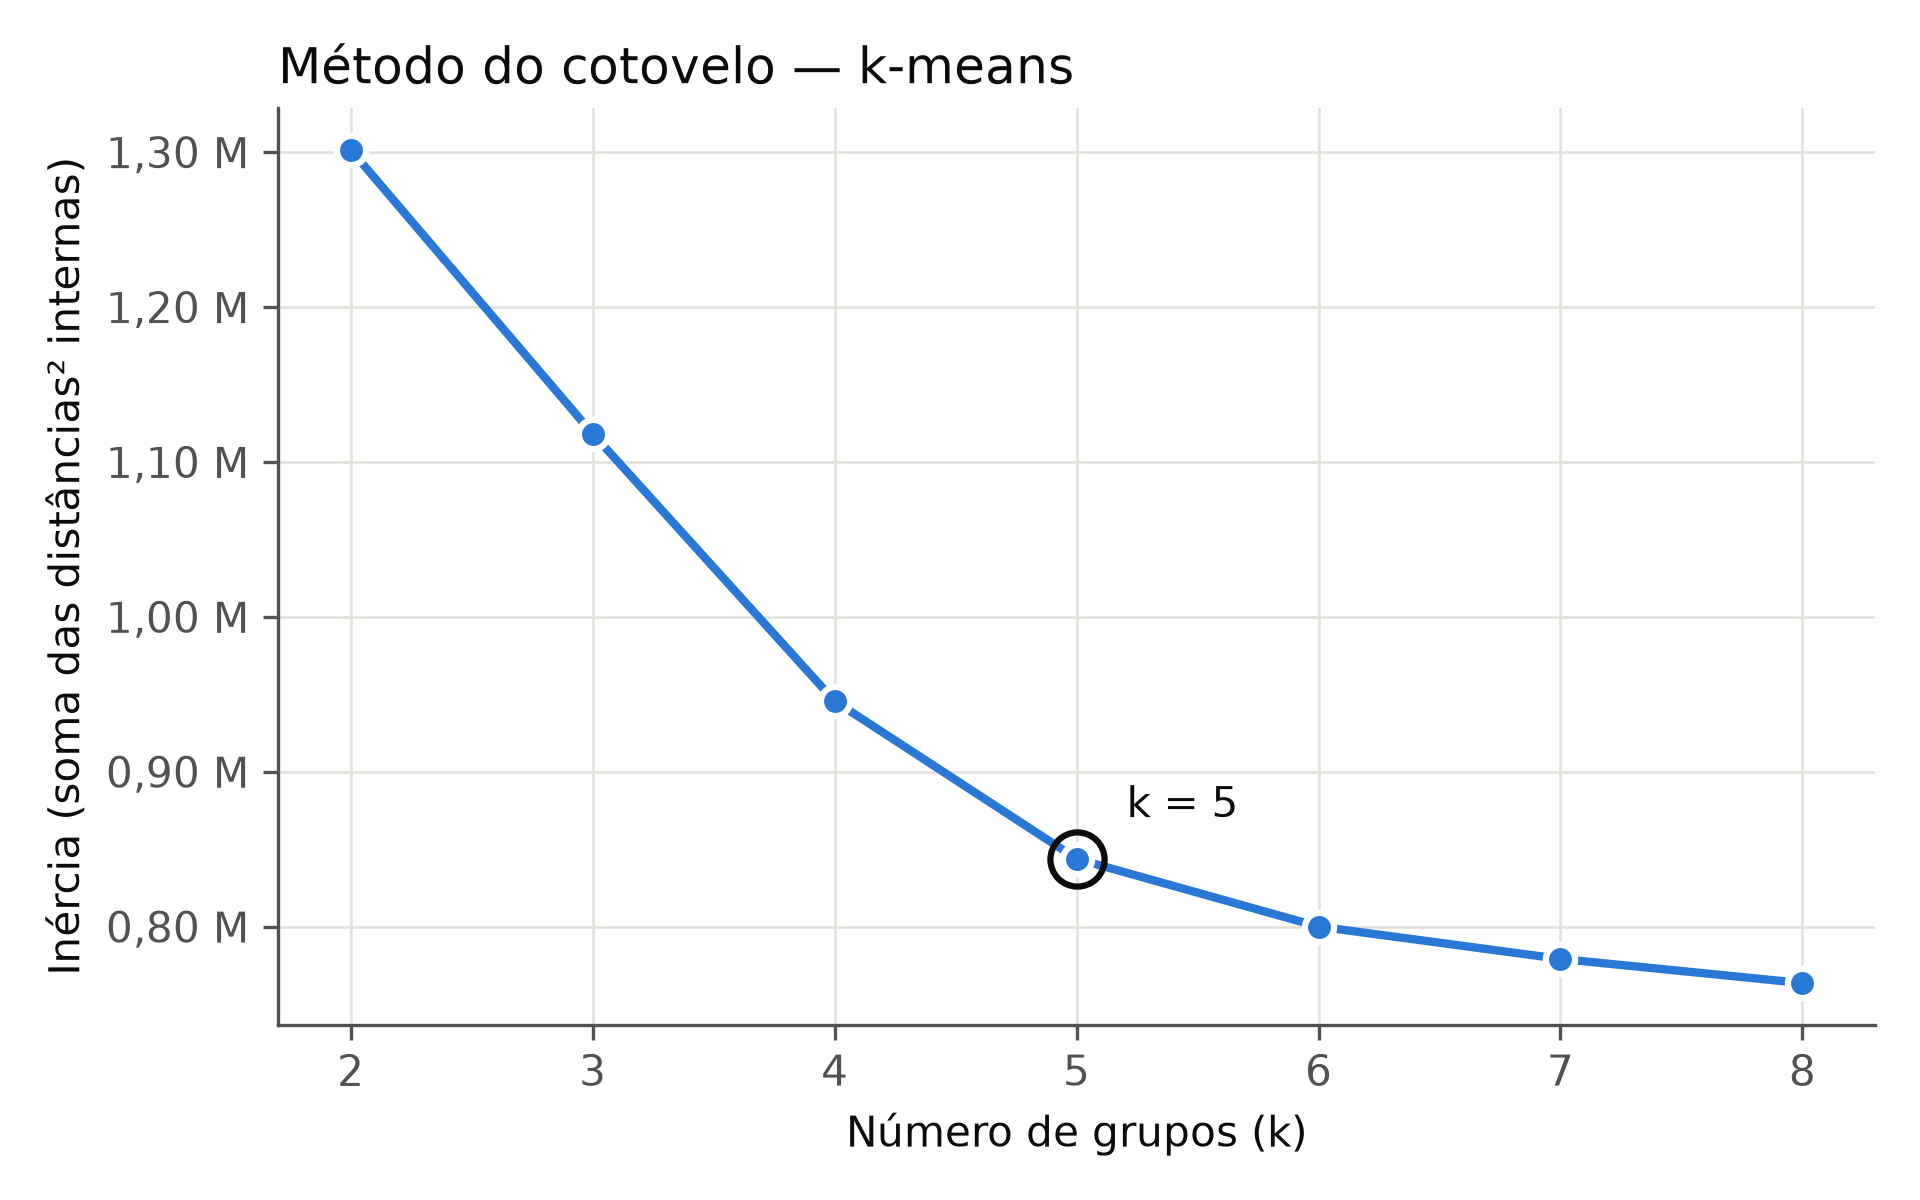
\includegraphics[width=0.62\linewidth]{fig_cotovelo.png}
  \caption{Método do cotovelo: inércia do k-means em função de $k$. O círculo marca o $k$ escolhido.}
  \label{fig:cotovelo}
\end{figure}

\begin{table}[htbp]
\caption{Inércia do k-means para cada valor de k.}
\label{tab:cotovelo}
\begin{tabular}{rll}
\toprule
k & Inércia & Queda em relação a k-1 \\
\midrule
2 & 1.301.489 & -- \\
3 & 1.118.218 & 14,1\% \\
4 & 945.655 & 15,4\% \\
5 & 843.806 & 10,8\% \\
6 & 800.037 & 5,2\% \\
7 & 779.142 & 2,6\% \\
8 & 763.533 & 2,0\% \\
\bottomrule
\end{tabular}
\end{table}


\subsection{Agrupamento hierárquico}

O dendrograma (Figura~\ref{fig:dendrograma}) mostra cinco ramos bem definidos abaixo da linha de corte para
$k=5$ (distância 372,3). Os tamanhos dos grupos (Tabela~\ref{tab:hierarquico}) são quase idênticos aos do
k-means (303, 145, 136, 140 e 77 amostras), o que já sugere que os dois métodos encontraram praticamente a
mesma divisão. Dois detalhes da árvore são importantes para a discussão: o ramo G3 se divide em dois a uma
distância de cerca de 290, pouco abaixo do corte, e os ramos G4 e G5 são os primeiros a se unir acima do
corte, a cerca de 450.

\begin{figure}[htbp]
  \centering
  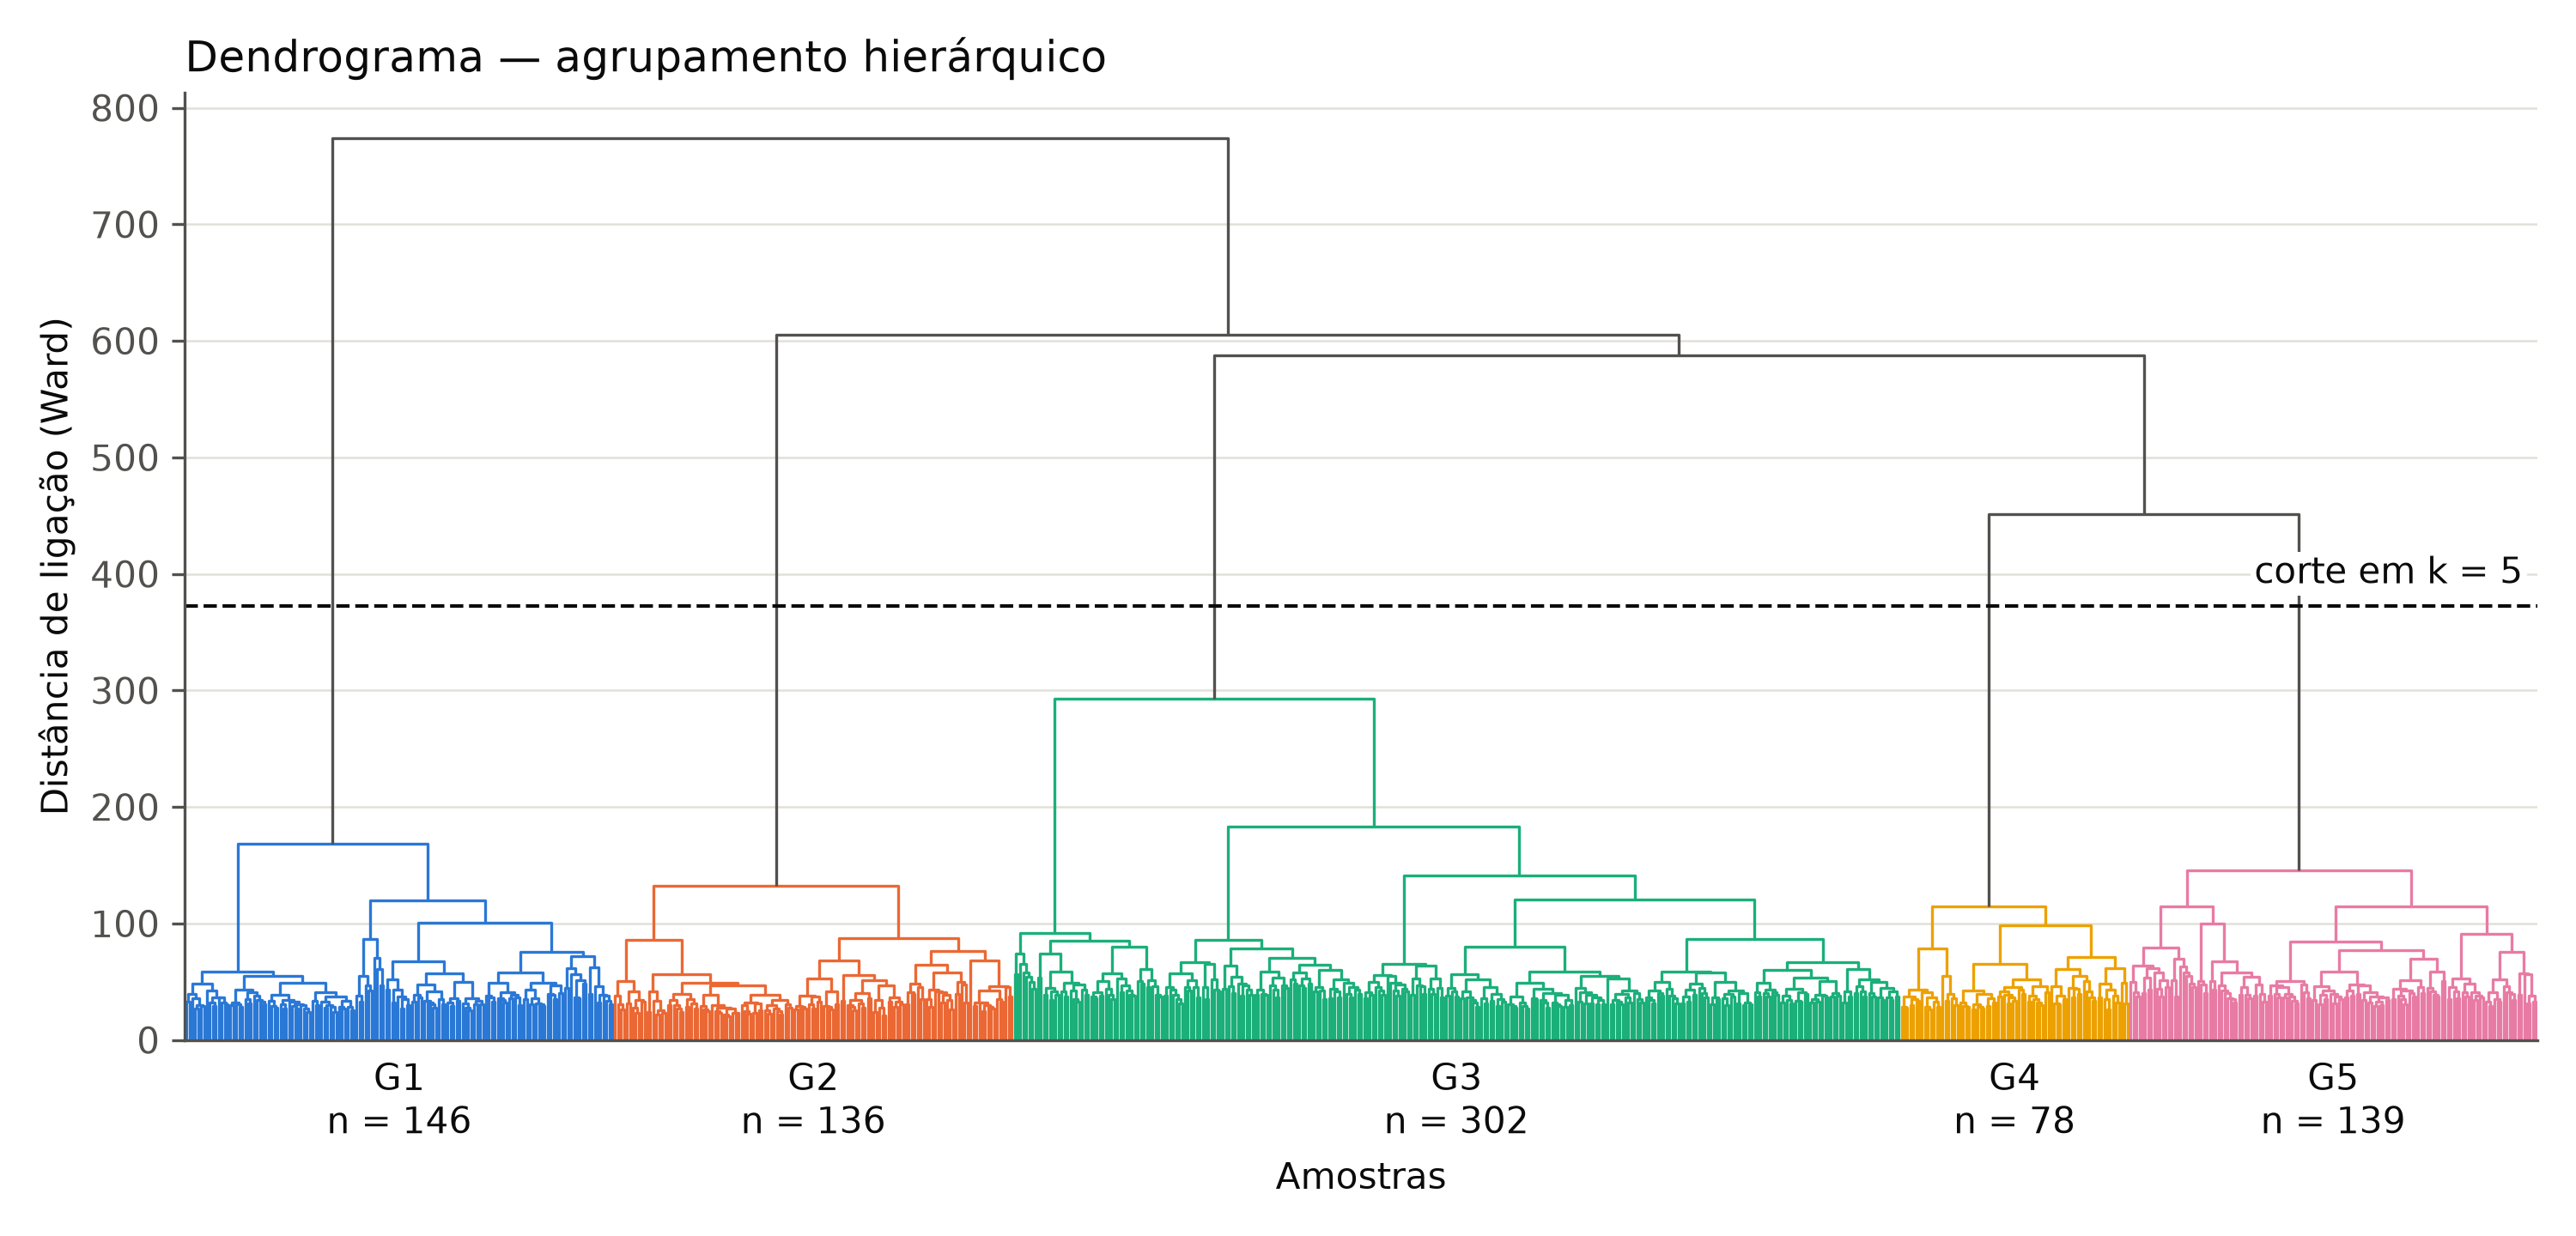
\includegraphics[width=\linewidth]{fig_dendrograma.png}
  \caption{Dendrograma do agrupamento hierárquico (Ward). Os ramos abaixo do corte em $k=5$ estão coloridos por grupo.}
  \label{fig:dendrograma}
\end{figure}

\begin{table}[htbp]
\caption{Tamanho dos grupos do agrupamento hierárquico (Ward) cortado em k = 5.}
\label{tab:hierarquico}
\begin{tabular}{lrl}
\toprule
Grupo & Amostras & Porcentagem \\
\midrule
G1 & 146 & 18,2\% \\
G2 & 136 & 17,0\% \\
G3 & 302 & 37,7\% \\
G4 & 78 & 9,7\% \\
G5 & 139 & 17,4\% \\
\bottomrule
\end{tabular}
\end{table}


\subsection{Comparação com os tipos de tumor}

As tabelas de contingência (Tabelas~\ref{tab:contingencia_kmeans} e~\ref{tab:contingencia_hierarquico})
mostram que cada grupo corresponde a um único tipo de tumor. A numeração dos grupos é arbitrária e diferente
em cada método: o G1 do k-means, por exemplo, corresponde ao G3 do hierárquico (BRCA). No k-means, só 4 das
801 amostras ficaram fora do grupo do seu tipo (1 KIRC e 2 LUAD no grupo de BRCA e 1 COAD no grupo de LUAD);
no hierárquico, só 2 (as duas amostras de LUAD no grupo de BRCA). Em ambos os casos, cada grupo tem pelo menos
99\% das amostras de um só tipo.

\sidebysidetables{tab_contingencia_kmeans.tex}{tab_contingencia_hierarquico.tex}

\subsection{Grupos na PCA}

A Figura~\ref{fig:pca} mostra os grupos no plano PC1 $\times$ PC2, que juntos explicam 32,0\% da variância
(Tabela~\ref{tab:pca}). KIRC e PRAD formam nuvens bem separadas, enquanto BRCA, LUAD e COAD ficam próximos, e
LUAD e COAD chegam a se sobrepor. Mesmo assim, os dois métodos separaram esses tipos quase perfeitamente,
porque o agrupamento usa os 2.000 genes, e não apenas os dois componentes do gráfico. As amostras circuladas,
cujo tipo real difere do tipo majoritário do grupo, ficam na fronteira entre as nuvens.

\begin{figure}[htbp]
  \centering
  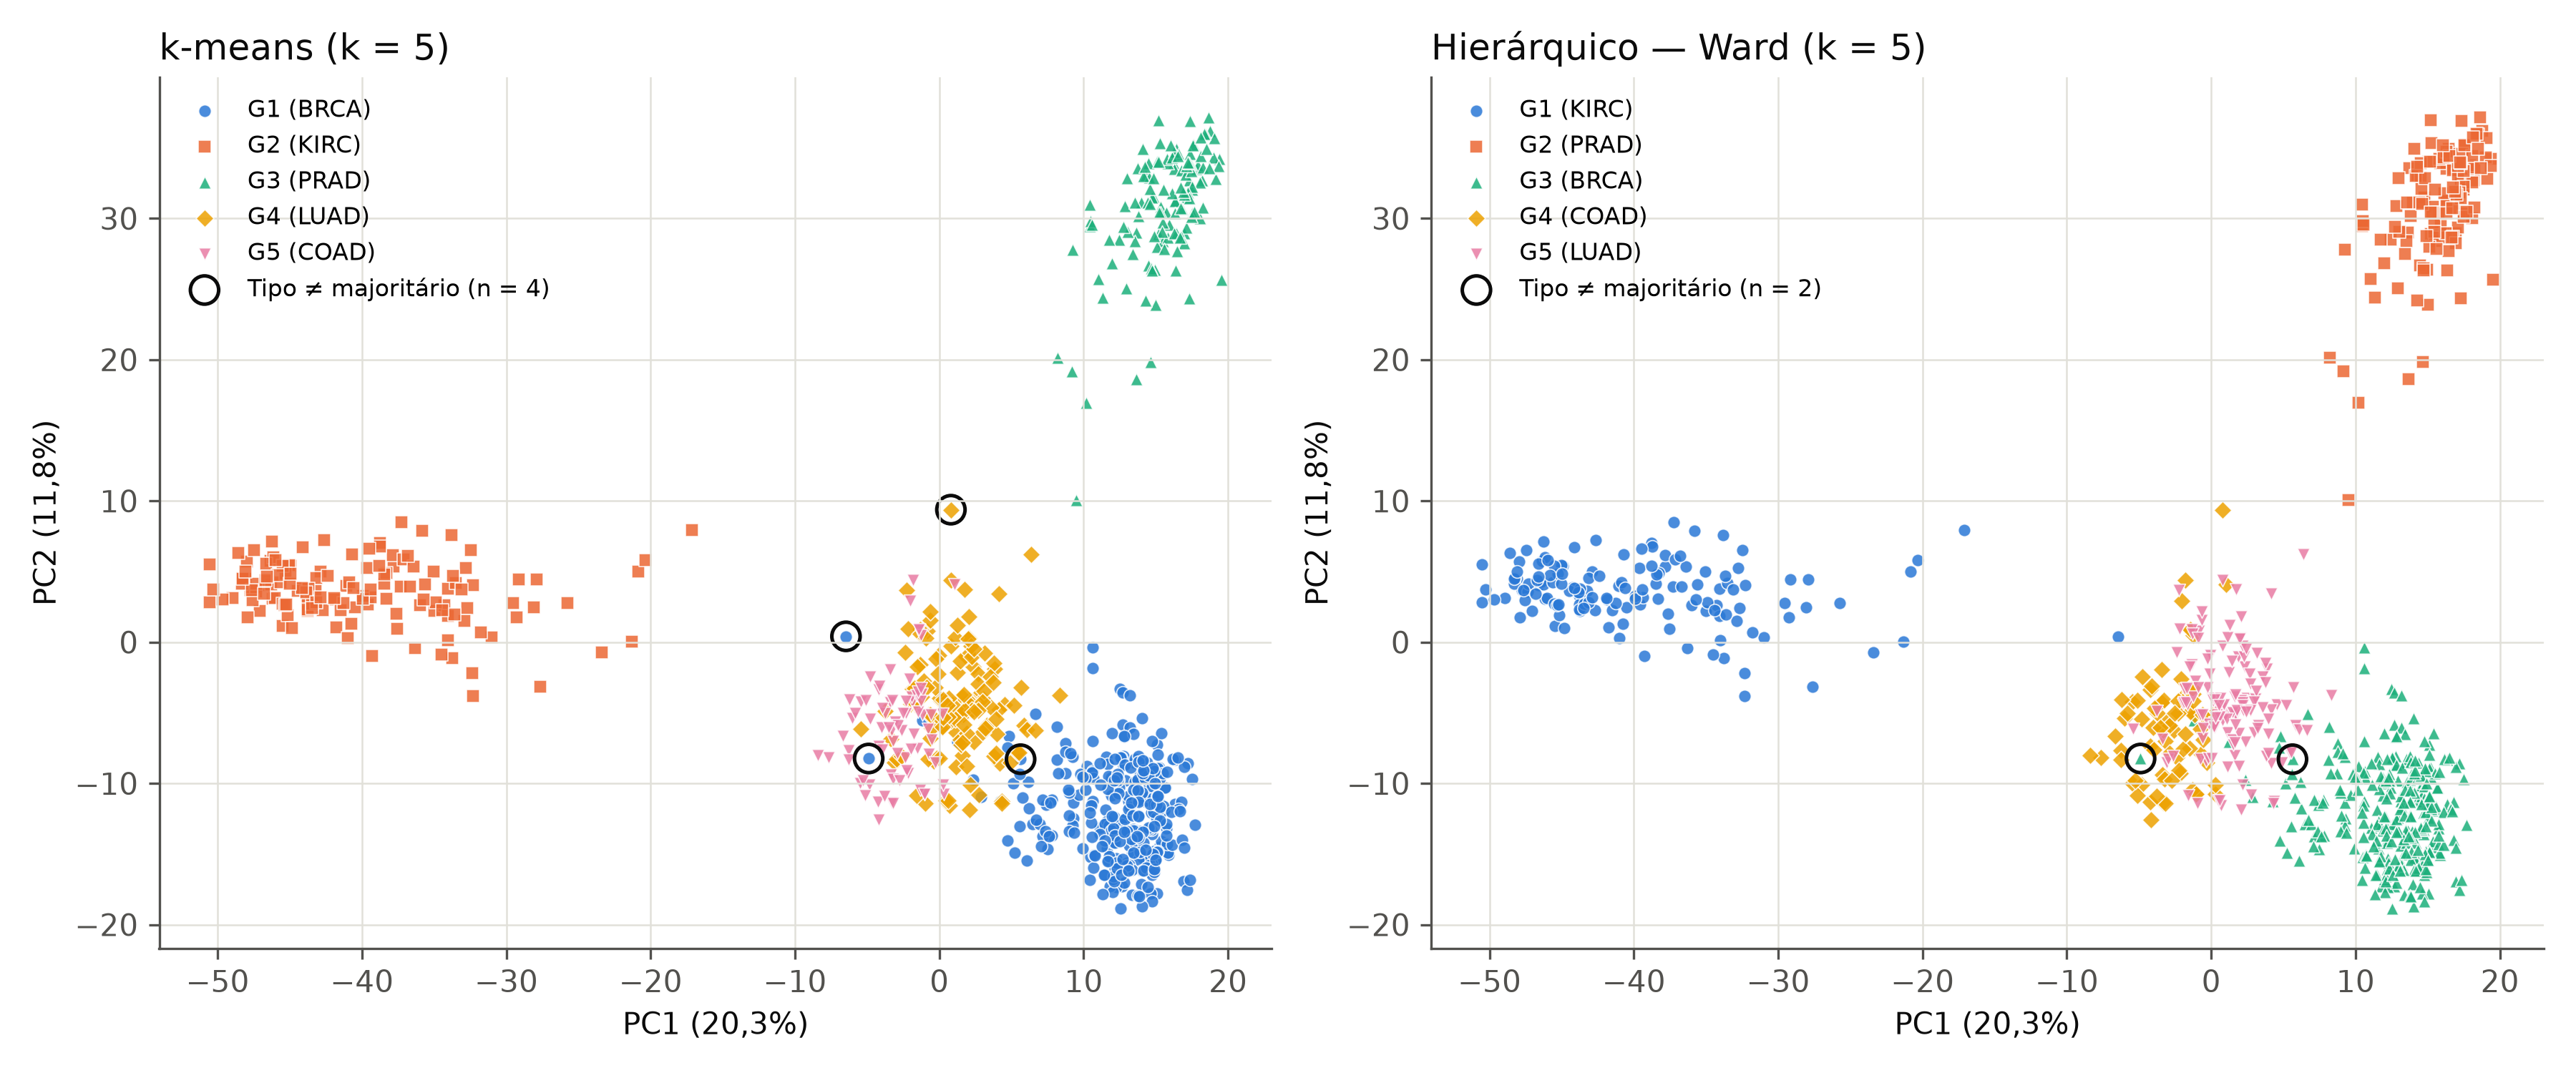
\includegraphics[width=\linewidth]{fig_pca_grupos.png}
  \caption{Amostras no plano PC1 $\times$ PC2, coloridas pelo grupo do k-means (esquerda) e do agrupamento
    hierárquico (direita). A legenda indica o tipo majoritário de cada grupo; os círculos marcam as amostras de
    outro tipo.}
  \label{fig:pca}
\end{figure}

\begin{table}[htbp]
\caption{Variância explicada pelos dois primeiros componentes principais.}
\label{tab:pca}
\begin{tabular}{lll}
\toprule
Componente & Variância explicada & Acumulada \\
\midrule
PC1 & 20,3\% & 20,3\% \\
PC2 & 11,8\% & 32,0\% \\
\bottomrule
\end{tabular}
\end{table}


% ---------------------------------------------------------------- 5
\section{Discussão}

\textbf{O método do cotovelo apontou $k=5$, que é o número real de tipos?}
Sim. Tanto o critério automático quanto a inspeção da curva indicam $k=5$. Ainda assim, a curva é suave e o
cotovelo não é um ponto muito marcado: olhando só o gráfico, $k=4$ ou $k=6$ também poderiam ser defendidos.
O método do cotovelo é uma heurística, e por isso foi útil combiná-lo com um critério objetivo.

\textbf{Algum tipo de tumor ficou dividido em dois grupos, ou dois tipos caíram no mesmo grupo?}
Não. Nos dois métodos, cada grupo corresponde a um único tipo e cada tipo está concentrado em um único grupo;
as exceções são amostras isoladas (4 no k-means e 2 no hierárquico, de 801). Isso indica que os perfis de
expressão dos cinco tumores são muito distintos, o que é esperado, já que eles vêm de tecidos diferentes.

\textbf{Por que um método de agrupamento pode encontrar uma divisão diferente da esperada sem estar errado?}
Porque o agrupamento não procura os tipos de tumor: ele procura a divisão que otimiza um critério geométrico
(no k-means e no Ward, a menor variância dentro dos grupos), e essa divisão depende de escolhas feitas antes,
como o valor de $k$, os genes usados, a padronização e o método de ligação. Os rótulos clínicos são apenas uma
das divisões biologicamente válidas dos dados. Se um tipo de tumor tiver subtipos moleculares, ou se tumores
de tecidos diferentes tiverem perfis de expressão parecidos, o método pode dividir um tipo ou juntar dois, e
esse resultado também descreve uma estrutura real dos dados. O nosso dendrograma mostra isso: com $k=6$ o ramo
de BRCA seria dividido em dois grupos, e com $k=4$ COAD e LUAD cairiam no mesmo grupo. Nenhuma dessas divisões
estaria errada; elas apenas mostram a estrutura dos dados em outra escala.

\section{Conclusão}

Sem usar os rótulos, o k-means e o agrupamento hierárquico de Ward, aplicados aos 2.000 genes de maior variância
padronizados, redescobriram os cinco tipos de tumor com no máximo 4 amostras fora do lugar, e o método do
cotovelo indicou o número correto de grupos. O resultado mostra que a expressão gênica separa bem esses tumores,
mas também que a divisão encontrada depende das escolhas do método: com outro $k$, os mesmos dados revelariam
uma estrutura diferente e igualmente válida.

\end{document}
